% !TEX root = ../../../main.tex
% 来源：中学数学实验教材·第三册（高中数学）
% 章节：二次函数 / 和二次函数有关的课题
% 原始文件：5.tex，行 2065-2079
% 类型：tikz
% ---
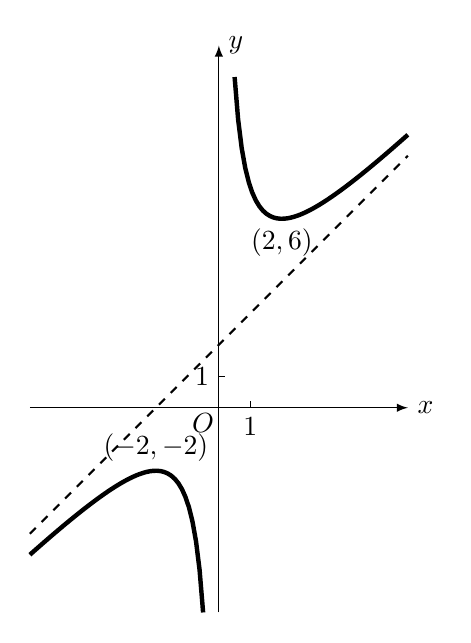
\begin{tikzpicture}[>=latex, scale=.4]
     \draw[->] (-6,0)--(6,0)node[right]{$x$};
    \draw[->] (0,-6.5)--(0,11.5)node[right]{$y$};   
    \draw [domain=-6:-.5, samples=50, ultra thick] plot(\x, {\x+4/\x+2});
    \draw [domain=.5:6, samples=50, ultra thick] plot(\x, {\x+4/\x+2});
    \draw [domain=-6:6, samples=5, dashed, thick] plot(\x, {\x+2});
    \foreach \x in {1}
    {
        \draw (\x,0)node[below]{\x}--(\x,.2);
        \draw(0,\x)node[left]{\x}--(.2,\x); 
    }
    \node at (-.5,-.5){$O$};
\node at (2,6)[below]{$(2,6)$};
\node at (-2,-2)[above]{$(-2,-2)$};
    \end{tikzpicture}
